\question
On lance trois dés (un rouge, un vert et un bleu) et on obtient un total de 11. Combien y a-t-il de façons différentes d'obtenir ce résultat ? 

\question
On répartit 11 billes entre trois boîtes (une rouge, une verte et une bleue), le nombre de billes par boîte n'étant pas limité. On caractérise une répartition par le nombre de billes présentes dans chaque boîte. On peut ne mettre aucune bille dans une boîte. Calculer le nombre de répartition différentes, selon que les billes sont discernables ou non. Comparer au cas précédent : qu'est-ce qui fait la différence ?

\question
On veut généraliser le calcul précédent au cas de $n$ billes et $N$ boîtes. En vous inspirant des trois dessins suivants, expliquer pourquoi ils représentent  tous le même système des $n$ billes dans $N$ boîtes, et en déduire que le nombre de répartition différentes cherché lorsque les billes sont indiscernables est donné par
$$
\frac{(N+n-1)!}{n! (N-1)!}
$$

\centerline{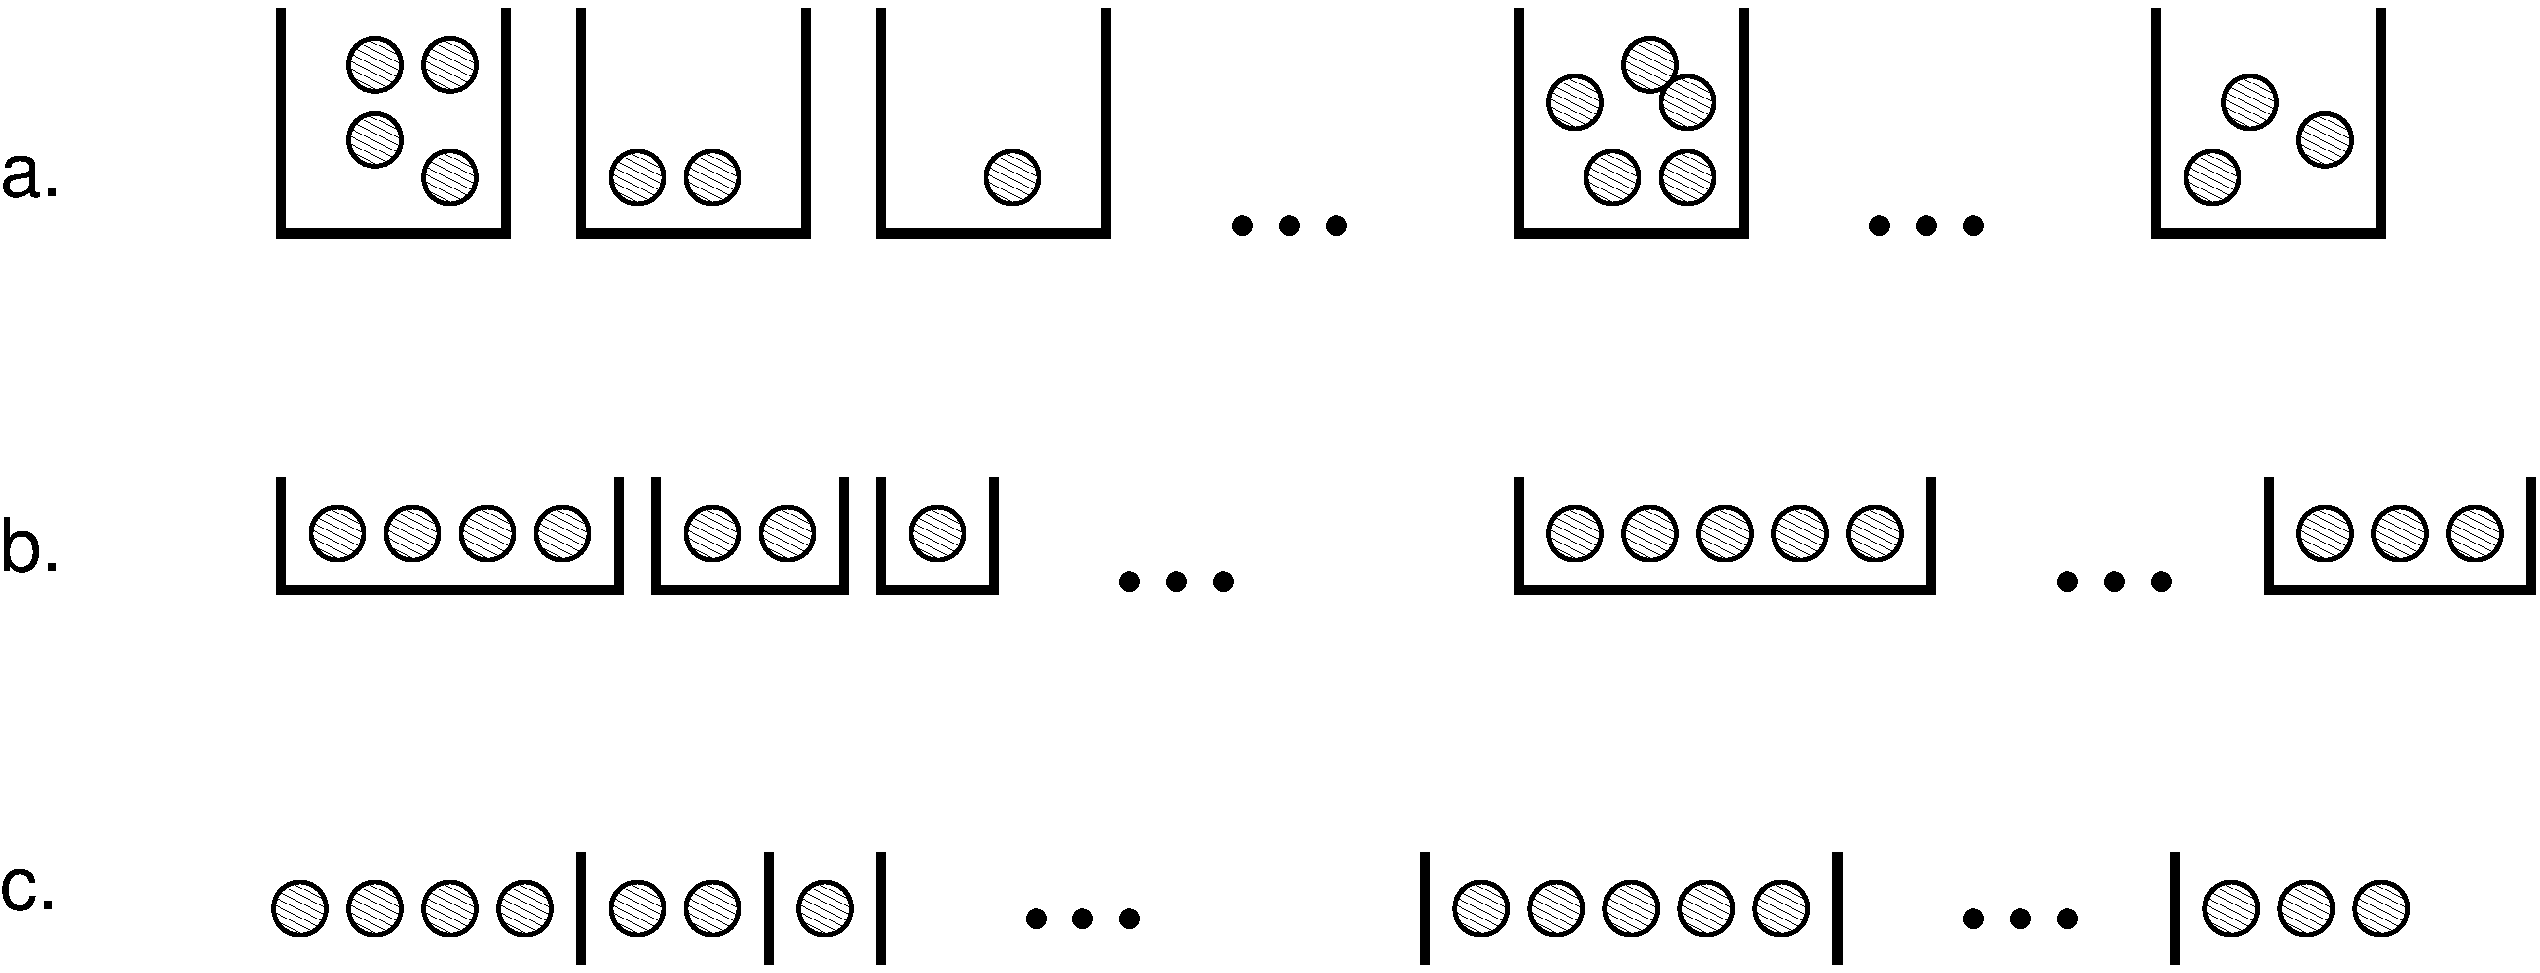
\includegraphics[height=.3\textwidth]{../Fig/Billes}}

\question
Comment est modifié ce résultat si les billes sont discernables ?

\question
Comment est modifié ce résultat si on ne peut pas mettre plus qu'une bille (indiscernable) par boîte ($N>n$) ?

\question
Qu'advient-il des résultats précédents lorsque $N\gg n$ ?
